\section{Results}
\label{sec:results}
The vulnerability discovery process in a bug bounty program is driven by the probability to find an additional bug given that $k$ bugs have already been discovered (i.e., the exhaustion process), and program managers aim to maximize $B_c$, the total number of bugs found. Our results show that the number of bugs discovered is a super-linear function of security researchers who have enrolled in the program (see Figure \ref{fig:scaling}A). While bounty programs benefit from the work of a large number of researchers, researchers overall benefit from diversifying their efforts across programs (see Figure \ref{fig:scalings_awards}C). This benefit is particularly tangible regarding the cumulative reward they can extract from their bug hunting activity. In particular, we illustrate how researchers take the strategic decision to enroll in a newly launched program, at the expense of existing ones they have formerly been involved in.
 
\subsection{Security researcher enrollment determines the success of a bug bounty program}
\label{sec:enrollment}

As presented on Figure \ref{fig:scaling}A, we find that the number $B_c$ of vulnerabilities discovered scales as $B_c \sim h^{\alpha}$ with $\alpha = 1.10(3)$ and $h$ the number of security researchers enrolled in a program. Since $\alpha > 1$, a bounty program benefits in a super-linear fashion from the enrollment of more researchers. This result is reminiscent of productive bursts and critical cascades of contributions in open source software development \cite{sornette2014much}: Each enrollment (i.e., {\it mother} event) initiates a cascade of vulnerability discoveries (i.e., {\it daughter} events) by the security researcher. Here, each cascade stems from a single security researcher (researchers mostly search bugs alone) and the nature of these cascades is captured at the aggregate level by their size as a random variable. As shown on Figure \ref{fig:scaling}B, the distribution of bounty discoveries per researcher and per program follows a power law tail $P(X>x) \sim 1/x^\gamma$  with $ \gamma = 1.63(7)$. The distribution is therefore heavy-tailed, but not extreme, as the first statistical moment (i.e., the mean) is well-defined (as a result of $ \gamma > 1$). Moreover, we observe an upper cut-off of the tail with $x_{max} \approx 400$ bounties. Thus, each enrollment of a security researcher in a program provides a statistically bounded amount of new bug discoveries. According to our data and analysis, there is no bug bounty ``czar" who could scoop a dominant portion of bugs. These results have somewhat counterintuitive organization design implications that we discuss later on.\\

\begin{figure}[ht]
\begin{center}
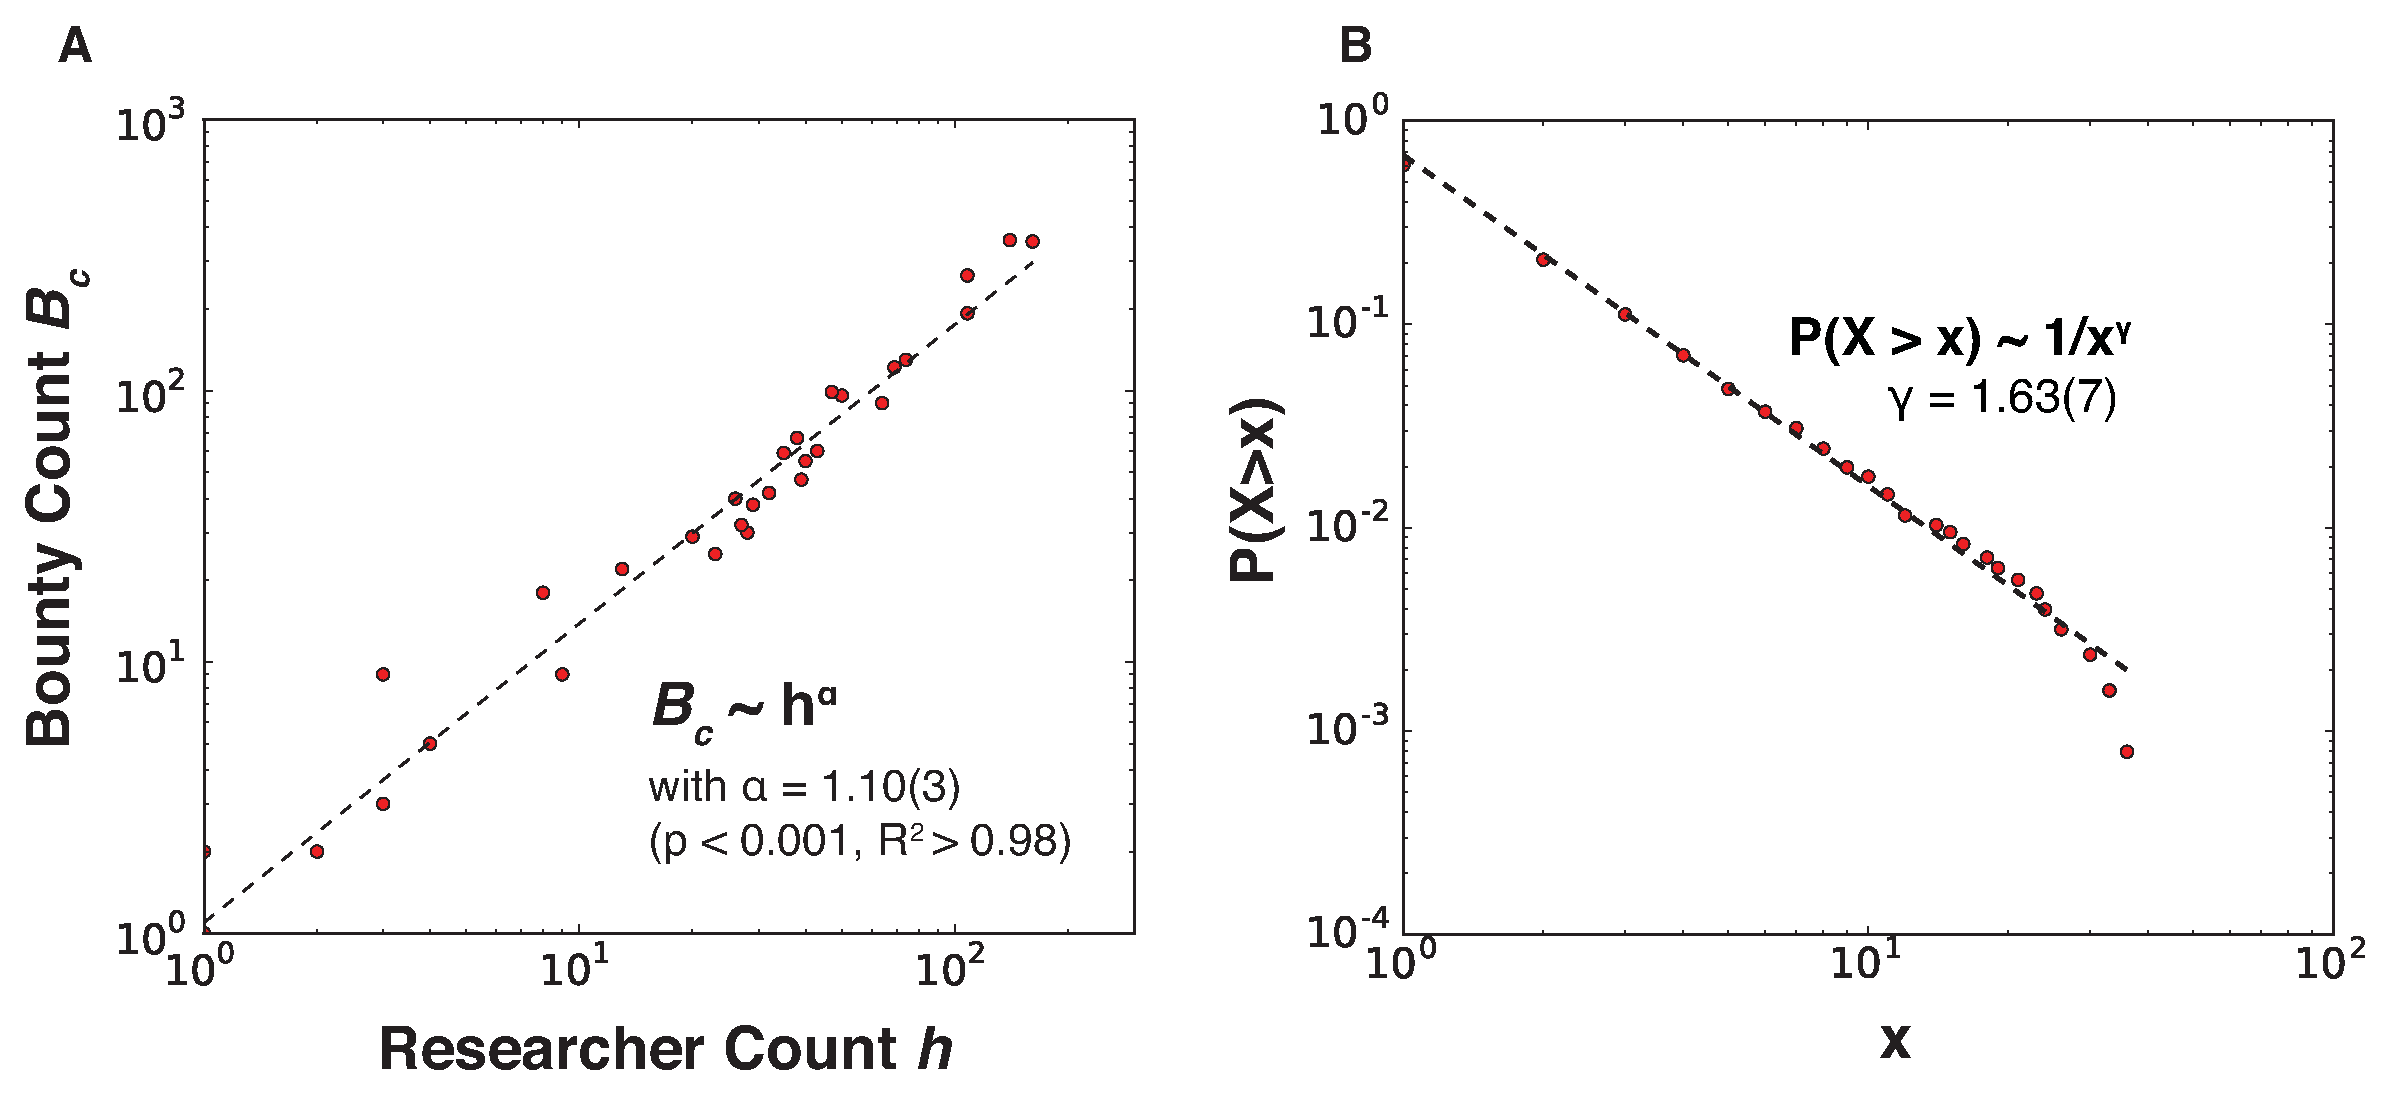
\includegraphics[width=12cm]{../figures/scaling.eps}
\caption{\footnotesize {\bf A.}  The number of bounty discoveries per program $B_c$ scales as $~h^{\alpha}$ with $\alpha = 1.10(3)$ and $h$ the number of security researchers enrolled in a program. Since $\alpha > 1$, a bounty programs benefits in a super-linear fashion to the enrollment of more researchers. {\bf B.} The tail distribution of bounty discoveries per researcher per program follows a power law distribution $P(X>x) \sim 1/x^\gamma$  with $1 < \gamma = 1.63(7) < 2$. The distribution is therefore relatively well bounded (with the first moment being well-defined). Furthermore, we observe an upper cut-off of the tail with $x_{max} \approx 400$ bounties. Thus, from {\bf A.} and {\bf B.} combined, we find that the number of vulnerabilities is mainly driven by the number of researchers enrolled in programs.}
\label{fig:scaling}
\end{center}
\end{figure}

 
\subsection{Security researchers are incentivized to diversify their contributions across bug bounty programs}
\label{sec:diversify}

For security researchers, the main metric is the expected cumulative payoff earned from the accumulation of bounty awards over all programs. This expected payoff is governed by the probability to find a given number of vulnerabilities and their associated payoff, as discussed in Section \ref{sec:method}. To fully understand the incentive mechanisms at work, we consider 3 perspectives: (i) the expected cumulative down-payment made by bug bounty program managers (see Figure \ref{fig:scalings_awards}A), the expected cumulative payoff from the viewpoint of a security researcher for (ii) one program (see Figure \ref{fig:scalings_awards}B), and for (iii) all programs (see Figure \ref{fig:scalings_awards}C).\\


\begin{figure}[ht]
\begin{center}
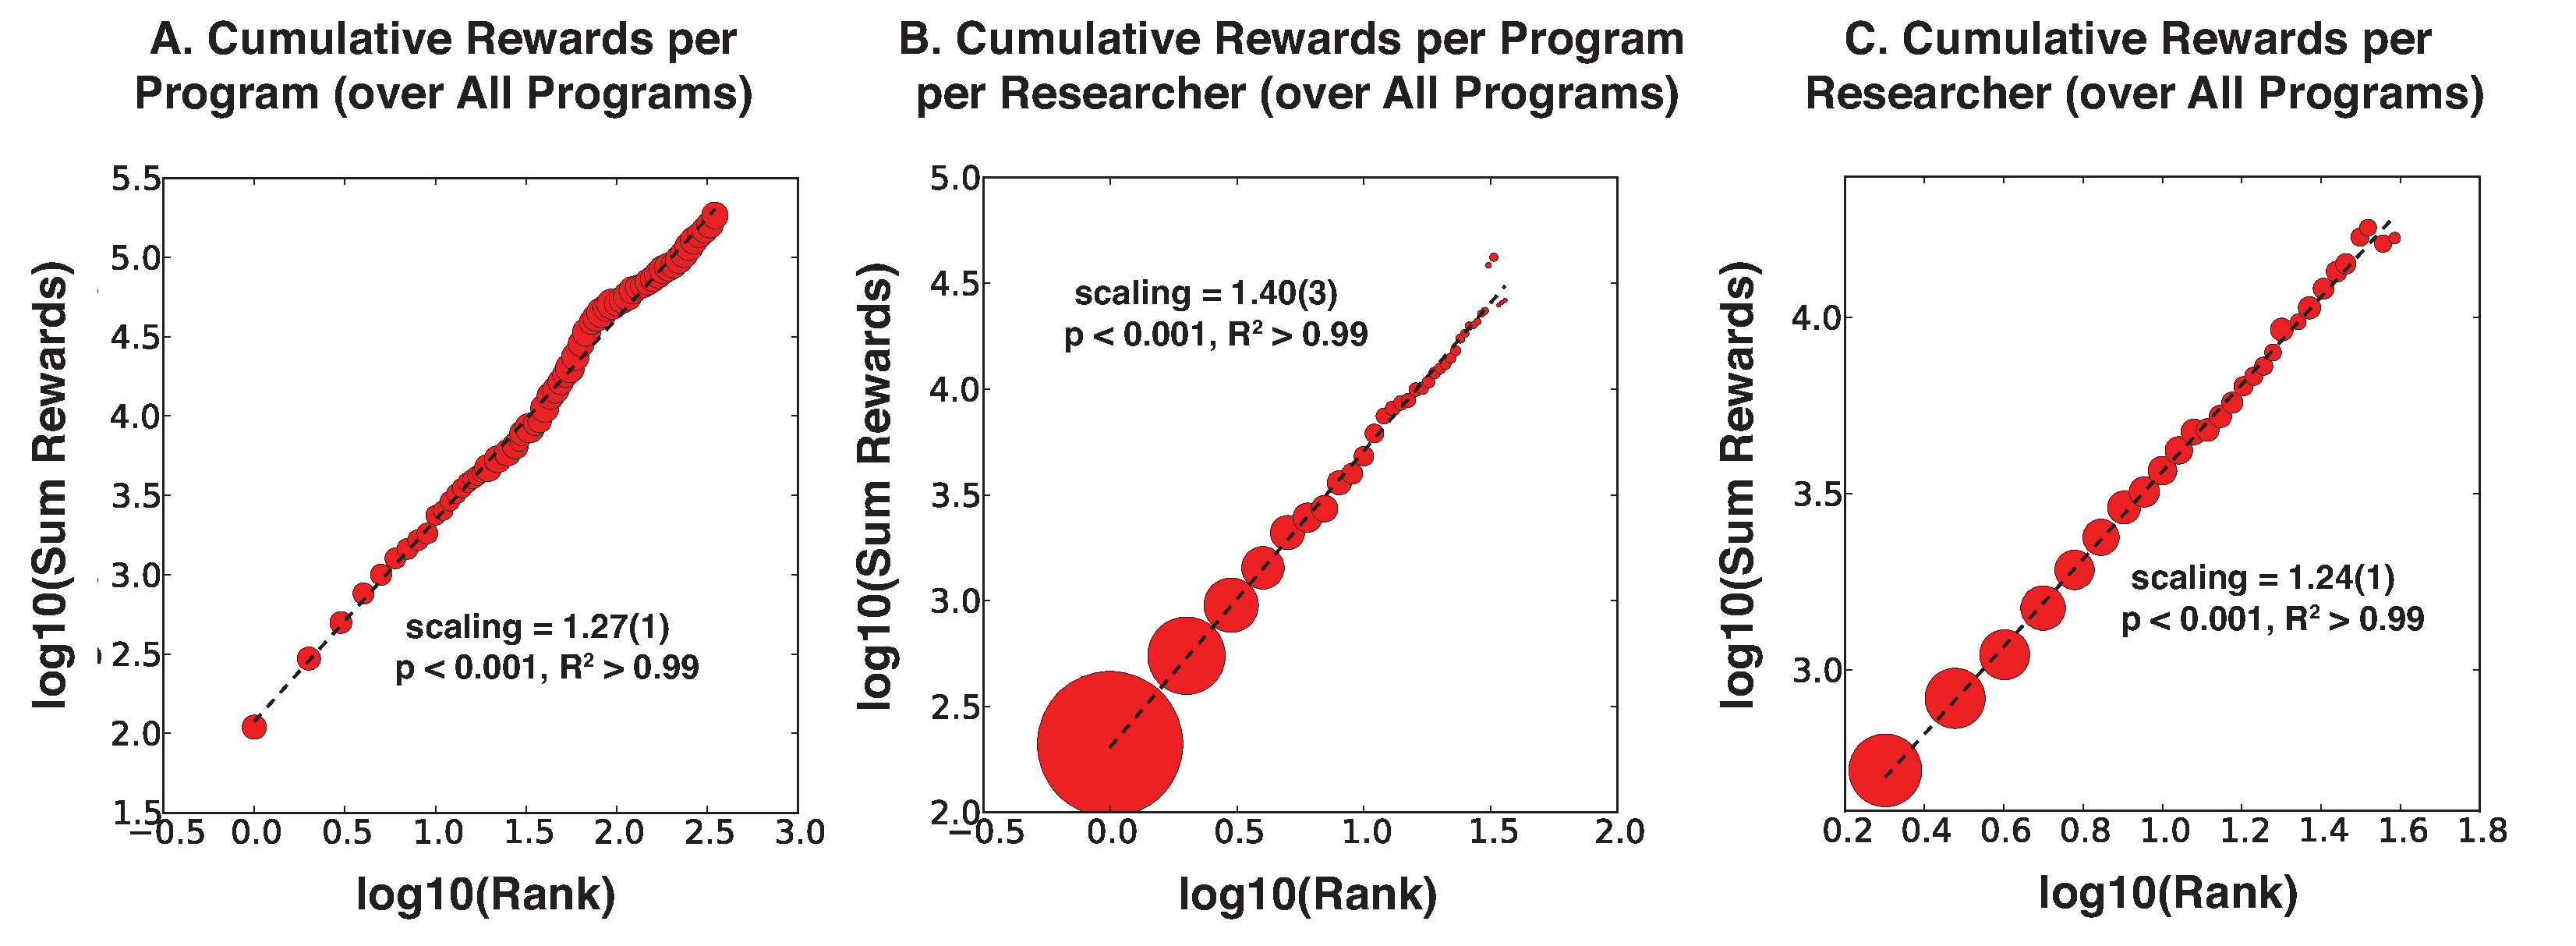
\includegraphics[width=12cm]{../figures/scalings_awards.eps}
\caption{{\bf A.} (Log-)binned cumulative down-payment per program over all public programs on the HackerOne platform, scales as $R_{k} \sim k^{1.27}$ ($ p < 0.001$, $R^2 > 0.99$), with $k$ the rank. Each log-bin shows the mean value and the circle sizes depict the number of values in each bin (i.e., the rank frequency). The super-linear {\it scaling} relationship between the cumulative reward and the rank shows that reward increases as a function of $k$. However, the frequency of vulnerabilities $P_k$ is only slightly upwards trended increasing as $ \sim k^{0.13}$ ($ p < 0.001$, $R^2 = 0.40$). {\bf B.} Considering the opposite figure from the viewpoint of researcher's expected payoff when enrolling in a single bug bounty program, the super-linear effect is much stronger ($R_{k} \sim k^{1.40}$ with $ p < 0.001$ and $R^2 > 0.99$). However, the frequency decays following a power law of the form $P_{k} \sim k^{-1.85}$ ($ p < 0.001$, $R^2 = 0.97$). {\bf C.} Over all bug bounty programs, security researchers have another expected payoff: the reward scaling is smaller ($R_{k} \sim k^{1.24}$ with $ p < 0.001$, $R^2 > 0.99$), yet the frequency of bug discoveries decays much slower as a function of rank $P_{k} \sim k^{-1.05}$ ($ p < 0.001$, $R^2 = 0.85$).}
\label{fig:scalings_awards}
\end{center}
\end{figure}

The average cumulative down-payment per program exhibits a super-linear scaling as $\sim k^{1.27}$ ($ p < 0.001$, $R^2 > 0.99$), while the frequency of vulnerabilities $P_k$ is only slightly upwards trended increasing as $ \sim k^{0.13}$ ($ p < 0.001$, $R^2 = 0.40$). The expected down-payment by bug bounty program managers therefore scales as $\sim k^{1.40}$. This is a considerable super-linear increase (as $k \rightarrow \infty$), which  casts questions on the long-term sustainability of bug bounty programs. \\

From the viewpoint of the security researcher and her expected payoff from a single bug bounty program, the increase of average cumulative reward ($R_{k} \sim k^{1.40}$) does not offset the fast decay of probability ($P_{k} \sim k^{-1.85}$) to find a vulnerability of rank $k$. The expected payoff therefore follows $\sim k^{-0.45}$, which clearly does not bring high incentives to explore in depth a bug bounty program. It is important to note however, that the bug bounty manager cannot fix $P_k$, which is a genuine feature of bug discovery by humans. To maintain positive individual incentives, the manager should set an incremental reward such that $R_k \sim k^{\alpha}$ with $\alpha > 1.40$, which in turn would worsen the down-payment function both in terms of incremental expenditures and in exploration of higher ranks. This approach does not consider possible individual human hard limits, preventing finding additional bugs. In that latter case, setting higher reward incentives would have no effect.\\

Security researchers tend to switch from one bounty program to another program \cite{zhao2014exploratory,zhao2015empirical}. The strategy can be assimilated to portfolio diversification \cite{goetzmann2008equity}. Over all bug bounty programs, security researchers have another much more favorable expected payoff: The reward scaling is smaller ($R_{k} \sim k^{1.24}$ with $ p < 0.001$, $R^2 > 0.99$), yet the frequency of bug discoveries decays much slower as a function of rank $P_{k} \sim k^{-1.05}$ ($ p < 0.001$, $R^2 = 0.85$). Therefore, over all bounty programs, security researchers have an increasing, yet marginally decreasing, incentive to explore higher ranks as $U_k \sim k^{0.19}$. In a nutshell, security researchers have an incentive to keep searching for bugs on a large variety of bug bounty programs.

\subsection{Influence of newly launched programs on researcher behaviors}
\label{ols}
As security researchers weigh their strategic choice to switch their attention from one program to another, the time factor is determinant because the expected payoff is dependent on the current vulnerability rank, which maps into the time dimension (i.e, the duration between two discoveries is drawn from a characteristic random variable, which is not considered here). While switching decision may be made by a researcher at any time, the most obvious moment is when a new program is being launched: Incentives shift suddenly, and security researchers may decide to abandon older programs at the expense of the new program. However, a number of factors may  influence their decision: The reputation of the organization launching the program (it brings more fame to submit a bug to e.g., Twitter compared to a less famous organization), the amount of reward, and the relative time between an old program and the newest one. Here, we aim to test  3 hypotheses:
\begin{itemize}
  \item {\bf H1:} An existing bounty program will receive less reports when more new programs are launched,
  \item {\bf H2:} An existing bounty program will receive less reports when bounty rewards provided by newly launched programs is higher,
  \item {\bf H3:} The number of newly launched programs has a larger impact on the contribution to older programs.
\end{itemize}


We start with a simple ordinary least square (OLS) regression model, which is specified as follows:
\begin{equation}
\label{reg_base}
V_{it} = \beta_0 + \beta_1 dP_t + \beta_2 T_{it} + \beta_3 A_{it} + \beta_4 B_{it} + \epsilon_{it}.
\end{equation}
$V_{it}$ is the number of vulnerability reports received by bounty program $i$ in the month $t$. $dP_t$ is the number of new programs launched in month $t$. Hypothesis {\bf H1} predicts that its coefficient ($\beta_1$) is negative. $T_{it}$ is the number of months since bounty program $i$ launched. We consider two control variables that could influence researcher's decision \cite{zhao2015empirical}. We first incorporate $A_i$ the log of the Alexa rank, which measures web traffic as a proxy of popularity for organization $i$. $B_i$ is the log of the average amount of bounty paid per bug by bounty program $i$. Both $A_i$ and $B_i$ are assumed to remain constant over time. Finally, $\epsilon_{it}$ is the unobservable error term. In models {\bf 2}-{\bf 4}, we extend the basic model (model {\bf 1}) to further study competition occurring between bounty programs. These alternative specifications include:

\begin{itemize}
  \item \textbf{Average bounty of newly launched programs:} Intuitively, if new programs offer higher rewards, they should attract more researchers from existing programs. We calculate the average bounty for all new programs in month $t$ as $NB_t$ in models {\bf 2}-{\bf 4}.
  
  \item \textbf{Interaction between $dP_t$ and $T_{it}$:} Conceivably, the effect of new programs on existing programs depends on certain characteristics of the latter, such as age. In particular, we ask if a new entrant has more negative effects on older programs compared to younger programs? To examine this, we consider an interaction term between the number of new programs ($dP_t$) and the age of the program ($T_{it}$) in models {\bf 3}-{\bf 4}. Hypothesis H3 predicts that its coefficient is negative.
  
  \item \textbf{Program fixed effect:} To better control for program-specific, time-invariant characteristics, e.g., the reputation among researchers, we add program fixed effect in model {\bf 4}. The addition of this fixed effect allows us to examine how bug discovery changes over time within each program $i$.
\end{itemize}

\begin{table}
	\centering
	\caption{Regression results.}
	\begin{tabular}{lcccc} \hline
		& (1) & (2) & (3) & (4) \\
		VARIABLES & $V_{it}$ & $V_{it}$ & $V_{it}$ & $V_{it}$ \\ \hline
		&  &  &  &  \\
		$dP_t$ & -1.235*** & -1.350*** & -2.310*** & -1.236** \\
		& (0.305) & (0.327) & (0.603) & (0.515) \\
		$A_i$ & -23.61*** & -23.72*** & -23.72*** & -7.188** \\
		& (2.140) & (2.156) & (2.152) & (3.473) \\
		$B_i$ & 16.64*** & 16.56*** & 16.75*** & -7.414 \\
		& (1.311) & (1.315) & (1.339) & (5.698) \\
		$T_{it}$ & -0.690 & -0.658 & -3.312*** & -3.758*** \\
		& (0.426) & (0.427) & (1.239) & (1.128) \\
		$B_{new,t}$ &  & -0.0445 & -0.0312 & -0.0321* \\
		&  & (0.0280) & (0.0277) & (0.0184) \\
		$T_{it} \times dP_t$ &  &  & 0.106** & 0.0755* \\
		&  &  & (0.0431) & (0.0406) \\
		Constant & 160.2*** & 170.4*** & 190.3*** & 136.5*** \\
		& (16.12) & (18.80) & (23.17) & (26.17) \\
		&  &  &  &  \\
		Observations & 1,212 & 1,212 & 1,212 & 1,212 \\
		R-squared & 0.314 & 0.316 & 0.319 & 0.647 \\
		Program FE & No & No & No & Yes \\ \hline
		\multicolumn{5}{c}{ Robust standard errors in parentheses} \\
		\multicolumn{5}{c}{ *** p$<$0.01, ** p$<$0.05, * p$<$0.1} \\
	\end{tabular}
	
	\label{tab:reg}
\end{table}

\noindent The regression results are shown in Table~\ref{tab:reg}. Consistent with our prediction in Hypothesis {\bf H1}, the coefficient of $dP_t$ is negative and statistically significant in all 4 specifications. {\it Ceteris paribus}, the launch of new programs reduces the number of vulnerabilities reported to existing programs. In other words, the entry of new programs indeed attracts researcher's attention away from existing programs, which is consistent with the fast decreasing expected payoff for individuals searching bugs for a specific program. Also, the average bounty paid by new programs ($B_{new,t}$) has a negative effect on existing programs as well, but the coefficient is only significant in model {\bf 4}. Again this result is consistent with the theory and Hypothesis {\bf H2}, as researchers have a higher incentive to switch to new programs, if they have more low-hanging fruits and higher bounty.\\

The interaction coefficients for term $T_{it} \times dP_t$ in models {\bf 3} and {\bf 4} are positive and statistically significant, so they do not support Hypothesis {\bf H3}. The result shows that the impact of newly launched programs depends on the age of the existing programs: Compared to younger programs, the negative impact of $dP_t$ is smaller for programs with a longer history, i.e., those with larger $T_{it}$. At first sight, this results may look at odds with the fact that individual expected payoff from a specific program decreases as a function of rank $k$, and presumably the older a program the more likely it has a high rank. Thus, the switching effect should be stronger. Perhaps our OLS regression model is limited in the sense that it does account for the absolute activity (which decreases very slowly as $t \rightarrow \infty$, as shown on Figure \ref{timeline}B), instead of the variation rate.

In consistent with previous research~\cite{zhao2015empirical}, the regression result also shows that a program with higher reputation ($A_i$) or higher bounty ($B_i$) is associated with more bugs received in a month. The regression result also shows that a program with longer age ($T_{it}$) is associated with less bugs found. This observation corresponds to the power law decay of bug submission observed following an initial shock (c.f., Figure \ref{timeline}B).

% (\textbf{TODO}: We can also test the robustness of the model by trying about alternative dependent variables, such as the the number of researchers that have submitted at least one report to program $i$ in month $t$.)